\documentclass{beamer}

%% \documentclass[handout]{beamer}
%% % use this with the [handout] option to create handouts for the audience
%% \usepackage{pgfpages}
%% \pgfpagesuselayout{2 on 1}[a4paper,border shrink=5mm]

\mode<presentation>
{
  \usetheme{Diku}
% set this to your preferences:
  \setbeamercovered{invisible}
%  \setbeamercovered{transparent}
}

\usepackage{graphicx}
\usepackage{epic}

\usepackage{amsmath}
\usepackage{amssymb}
\usepackage{amsthm}

\newcommand{\basetop}[1]{\vtop{\vskip-1ex\hbox{#1}}}
\newcommand{\source}[1]{\let\thefootnote\relax\footnotetext{\scriptsize\textcolor{kugray1}{Source: #1}}}

% for coloured code citation in text:
\usepackage{fancyvrb}

%%%%%%%%%%%%%%%%%%%%%%%%%%%%%%%%%
%%%%%    code sections   %%%%%%%%
%%%%%%%%%%%%%%%%%%%%%%%%%%%%%%%%%

% code highlighting commands in own block
\DefineVerbatimEnvironment{code}{Verbatim}{fontsize=\scriptsize}
\DefineVerbatimEnvironment{icode}{Verbatim}{fontsize=\scriptsize}

% Fancy code with color commands:
\DefineVerbatimEnvironment{colorcode}%
        {Verbatim}{fontsize=\scriptsize,commandchars=\\\{\}}

%%%%%%%%%%%%%%%%%%%%%%%%%%%%%%%%%%
%%%%%    some coloring    %%%%%%%%

\definecolor{Red}{RGB}{220,50,10}
\definecolor{Blue}{RGB}{0,51,102}
\definecolor{Yellow}{RGB}{102,51,0}
\definecolor{Orange}{RGB}{178,36,36}
\definecolor{Grey}{RGB}{180,180,180}
\definecolor{Green}{RGB}{20,120,20}
\definecolor{Purple}{RGB}{160,50,100}
\newcommand{\red}[1]{\textcolor{Red}{{#1}}}
\newcommand{\blue}[1]{\textcolor{Blue}{{#1}}}
\newcommand{\yellow}[1]{\textcolor{Yellow}{{#1}}}
\newcommand{\orange}[1]{\textcolor{Orange}{{#1}}}
\newcommand{\grey}[1]{\textcolor{Grey}{{#1}}}
\newcommand{\green}[1]{\textcolor{Green}{{#1}}}
\newcommand{\purple}[1]{\textcolor{Purple}{{#1}}}




% use "DIKU green" from our color theme for \emph
\renewcommand{\emph}[1]{\textcolor{structure}{#1}}
% use some not-too-bright red for an \emp command
\definecolor{DikuRed}{RGB}{130,50,32}
\newcommand{\emp}[1]{\textcolor{DikuRed}{ #1}}
\definecolor{CosGreen}{RGB}{10,100,70}
\newcommand{\emphh}[1]{\textcolor{CosGreen}{ #1}}
\definecolor{CosBlue}{RGB}{55,111,122}
\newcommand{\emphb}[1]{\textcolor{CosBlue}{ #1}}
\definecolor{CosRed}{RGB}{253,1,1}
\newcommand{\empr}[1]{\textcolor{CosRed}{ #1}}

\newcommand{\mymath}[1]{$ #1 $}
\newcommand{\myindx}[1]{_{#1}}
\newcommand{\myindu}[1]{^{#1}}

\newtheorem{mydef}{Definition}
\newtheorem{mytheo}{Theorem}
\newtheorem{mylemma}{Lemma}


%%%%%%%%%%%%%%%%%%%%

\title[Intro]{List Homomorphism}

\author[C.~Oancea]{Cosmin E. Oancea\\{\tt [cosmin.oancea]@diku.dk}}

\institute{Department of Computer Science (DIKU)\\University of Copenhagen}


\date[Sept 2015]{September 2015 PMPH Lecture Notes}


\begin{document}

\titleslide


%%%%%%%%%%%%%%%%%%%%%%%%%%%%%%%%%%%%%%%%%%%%%%%%%%%%%%%%%%%%%%%%%%%%%%
%%%%%%%%%%%%%%%%%%%%%%%%%%%%%%%%%%%%%%%%%%%%%%%%%%%%%%%%%%%%%%%%%%%%%%
%%%%%%%%%%%%%%%%%%%%%%%%%%%%%%%%%%%%%%%%%%%%%%%%%%%%%%%%%%%%%%%%%%%%%%
%\begin{frame}[fragile]
%	\tableofcontents
%\end{frame}

%%%%%%%%%%%%%%%%%%%%%%%%%%%%%%%%%%%%%%%%%%%%%%%%%%%
%%%%%%%%%%%%%%%%%%%%%%%%%%%%%%%%%%%%%%%%%%%%%%%%%%%
%%%%%%%%%%%%%%%%%%%%%%%%%%%%%%%%%%%%%%%%%%%%%%%%%%%

\begin{frame}[fragile,t]
\frametitle{Intended Learning Outcomes}

List Homomorphism: a way of writing inherently-parallel programs.
\bigskip

\begin{itemize}
    \item explain Moore's law and discuss why the hardware parallelism (number of cores/processors) 
            is likely to increase exponentially.\bigskip
    \item explain what a list-homomorphic program is, and 
    \item be able to apply it to build programs.\bigskip
    \item illustrate and apply the 1$^{st}$ Theorem of List Homomorphism 
                to transform said programs into inherently parallel ones.
\end{itemize}
\end{frame}


\section{Path to Higher Performance: Increase Hardware Parallelism}

\begin{frame}[fragile,t]
\frametitle{Trend towards Ever-Increasing Hardware Parallelism}

\emp{\bf Moore's Law (1960s)}
\begin{itemize}
        \item ``Number of transistors in a dense integrated circuit doubles approximatively 
                    every two years.''\pause\bigskip
        \item Rephrased as:\medskip
            \begin{itemize}
                \item computing power doubles every 19-24 months, and 
                \item cost effectiveness ({\tt performance/cost}) keeps pace.
            \end{itemize}\bigskip
\end{itemize}

\emp{\bf Brief History}
\begin{itemize}
        \item \emph{ICPP, ISCA (1980/90s): parallel architectures popular topic.}\bigskip
                %\\Demise of SingleCPU System: inevitable \& fast approaching.\bigskip

        \item \alert{Whatever happened? Mid90 Killer-Micro:}\pause
        \begin{itemize}
            \item path of least resistance: ever increasing the speed of Single CPU
            %\item Muscled processors executing 100s instructions/cycle.
            \item Commercial arena: multiprocessors just an uniprocessor extension.
        \end  {itemize}\bigskip

        \item \emph{What Changed?} Multiprocessors Trend: Academia \& Industry:
        \begin{itemize}
            \item \emph{power complexity} $P_{dynamic} \sim Freq^3$. \alert{Example!}\pause
            \item \emph{Memory WALL}: ever-increasing performance gap between 
                                        processor \& memory 
        \end  {itemize}\bigskip

%       \item \emph{All Future Architectures adopt some form of massive parallelism!}
\end{itemize}

\end{frame}

\begin{frame}[fragile,t]
\frametitle{Processor: Clock Frequency/Rate}

1990-2004: clock rate has increased exponentially.

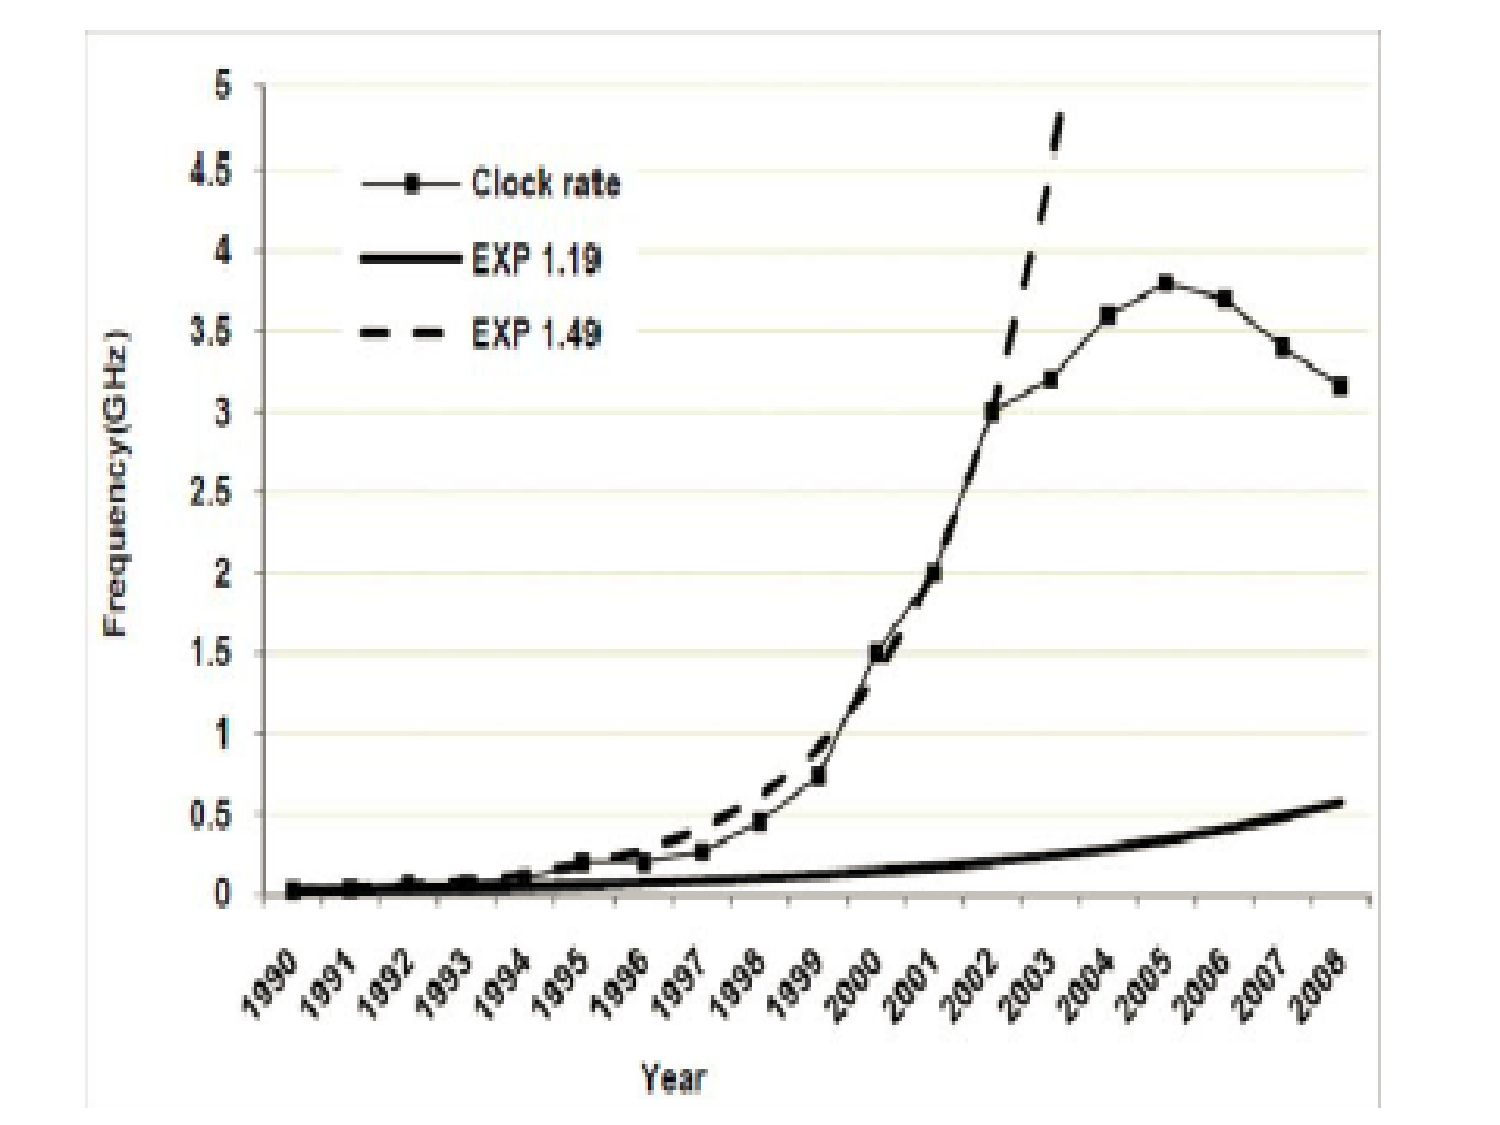
\includegraphics[width=47ex]{Figures/L1/FreqGraph}

2004: Intel cancels Pentium4 @4Ghz and shifts focus to multi-cores.

\end{frame}


\begin{frame}[fragile,t]
\frametitle{Memory Wall? Which Memory Wall??}

\begin{columns}
\column{0.65\textwidth}
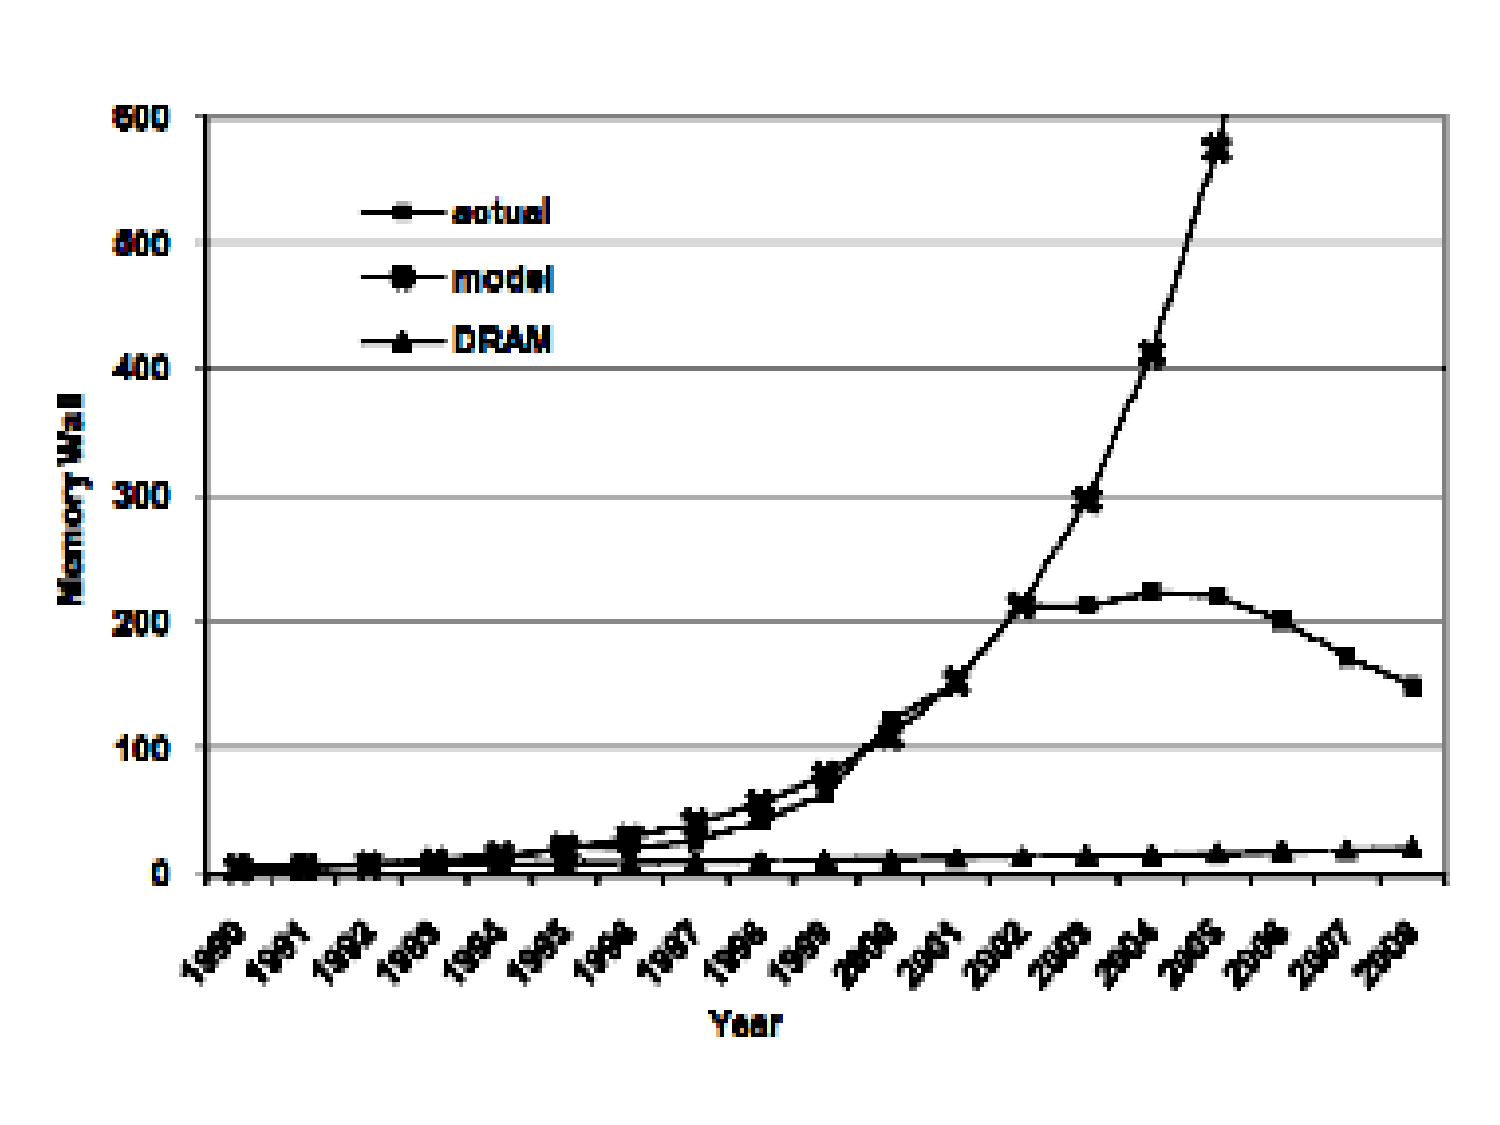
\includegraphics[width=50ex]{Figures/L1/MemWall}
\column{0.3\textwidth}
\begin{scriptsize}
\begin{itemize}
\item {\tt MemoryWall = mem\_cycle/ proc\_cycle} \smallskip
\item[1990] {\tt MemoryWall = 4} (25MHz,150ns)
\item[2002] exponential growth {\tt MemoryWall = 200} 
\item Stalled since then.
\end{itemize}
\end{scriptsize}
\end{columns}

\end{frame}


\begin{frame}[fragile,t]
\frametitle{Biggest Challenge For Parallel Hardware}

\bigskip

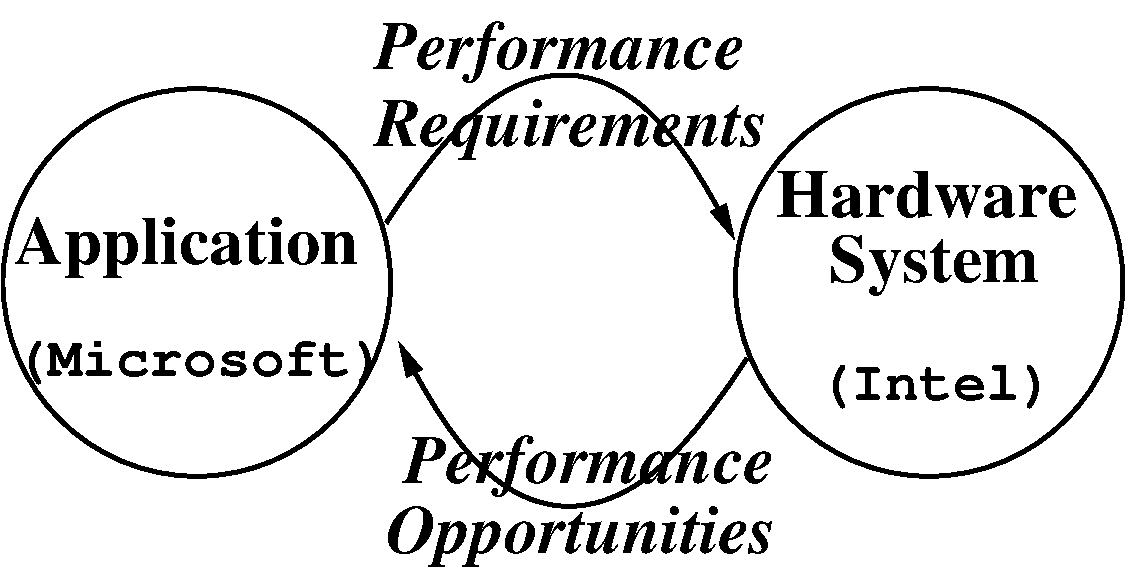
\includegraphics[width=29ex]{Figures/L1/Synergy}
\bigskip\pause


\emp{Important Juncture:}\medskip
\begin{itemize}
            \item \emph{Trend Today: the number of cores grows exponentially.}\medskip
            \item \alert{Biggest Challenge: develop efficient Massively-Parallel Software!}\medskip
            \item think programs with parallelism in mind rather 
                    than hack \alert{some} parallelism out of a sequential implementation.
\end  {itemize}
\end{frame}


\section{List Homomorphisms (LH)}

\begin{frame}[fragile]
	\tableofcontents[currentsection]
\end{frame}

\begin{frame}[fragile,t]
\frametitle{Shape of a List-Homomorphic Program (LH)}

Realm of finite lists:
\begin{itemize}
    \item {\tt ++} denotes list concatenation:\\
    {\tt [1, 2, 3] ++ [4, 5, 6, 7] $\equiv$ [1, 2, 3, 4, 5, 6, 7]}
    \item empty list {\tt []} is the neutral element:
        {\tt [] ++ x $\equiv$ x ++ [] $\equiv$ x}
\end{itemize}
\bigskip

\emp{\bf LH: a special form of divide and conquer programming:}
\begin{columns}
\column{0.45\textwidth}
\begin{colorcode}[fontsize=\small]
h( [ ] )   = e
h( [x] )   = f(x)
h( x ++ y) = h(x) \mymath{\odot} h(y)
\end{colorcode}
\pause
\alert{A well-defined program requires that no matter how 
the input list is partitioned into {\tt x ++ y}, the result is the same!}
\column{0.45\textwidth}
\begin{colorcode}[fontsize=\small]
\blue{--computes the length of a list,}
\blue{--(how many elements a list has)}
len :: [T] -> Int
len([ ])    = \alert{???}
len([x])    = \alert{???}
len(x ++ y) = len(x) \alert{???} len(y)
\end{colorcode}
\end{columns}

\end{frame}

\begin{frame}[fragile,t]
\frametitle{Shape of a List-Homomorphic Program (LH)}

Realm of finite lists:
\begin{itemize}
    \item {\tt ++} denotes list concatenation:\\
    {\tt [1, 2, 3] ++ [4, 5, 6, 7] $\equiv$ [1, 2, 3, 4, 5, 6, 7]}
    \item empty list {\tt []} is the neutral element:
        {\tt [] ++ x $\equiv$ x ++ [] $\equiv$ x}
\end{itemize}
\bigskip

\emp{\bf LH: a special form of divide and conquer programming:}
\begin{columns}
\column{0.45\textwidth}
\begin{colorcode}[fontsize=\small]
h( [ ] )   = e
h( [x] )   = f(x)
h( x ++ y) = h(x) \mymath{\odot} h(y)
\end{colorcode}
\alert{A well-defined program requires that no matter how 
the input list is partitioned into {\tt x ++ y}, the result is the same!}
\column{0.45\textwidth}
\begin{colorcode}[fontsize=\small]
-- one :: Int -> Int
-- one(x) = 1
len :: [T] -> Int
len([ ])    = \emp{0}
len([x])    = \emp{one}(x) \blue{-- \mymath{\equiv} 1}
len(x ++ y) = len(x) \emp{+} len(y)
\end{colorcode}
\end{columns}

\end{frame}


\begin{frame}[fragile,t]
\frametitle{Shape of a List-Homomorphic Program (LH)}

Realm of finite lists:
\begin{itemize}
    \item {\tt ++} denotes list concatenation:\\
    {\tt [1, 2, 3] ++ [4, 5, 6, 7] $\equiv$ [1, 2, 3, 4, 5, 6, 7]}
    \item empty list {\tt []} is the neutral element:
        {\tt [] ++ x $\equiv$ x ++ [] $\equiv$ x}
\end{itemize}
\bigskip

\emp{\bf LH: a special form of divide and conquer programming:}
\begin{columns}
\column{0.45\textwidth}
\begin{colorcode}[fontsize=\small]
h( [ ] )   = e
h( [x] )   = f(x)
h( x ++ y) = h(x) \mymath{\odot} h(y)
\end{colorcode}
\alert{A well-defined program requires that no matter how 
I partition the input list into {\tt x ++ y} I get the same result!}
\column{0.52\textwidth}
\begin{colorcode}[fontsize=\small]
\blue{--Assume p :: T -> Bool given,}
\blue{--compute whether all elements of}
\blue{--a list satisfy predicate p.}
all\mymath{\myindx{p}} :: [T] -> Bool
all\mymath{\myindx{p}}([ ])  = \alert{???}
all\mymath{\myindx{p}}([x])  = \alert{???} 
all\mymath{\myindx{p}}(x++y) = all\mymath{\myindx{p}}(x) \alert{???} all\mymath{\myindx{p}}(y)
\end{colorcode}
\end{columns}

\end{frame}


\begin{frame}[fragile,t]
\frametitle{Shape of a List-Homomorphic Program (LH)}

Realm of finite lists:
\begin{itemize}
    \item {\tt ++} denotes list concatenation:\\
    {\tt [1, 2, 3] ++ [4, 5, 6, 7] $\equiv$ [1, 2, 3, 4, 5, 6, 7]}
    \item empty list {\tt []} is the neutral element:
        {\tt [] ++ x $\equiv$ x ++ [] $\equiv$ x}
\end{itemize}
\bigskip

\emp{\bf LH: a special form of divide and conquer programming:}
\begin{columns}
\column{0.45\textwidth}
\begin{colorcode}[fontsize=\small]
h( [ ] )   = e
h( [x] )   = f(x)
h( x ++ y) = h(x) \mymath{\odot} h(y)
\end{colorcode}
\alert{A well-defined program requires that no matter how 
I partition the input list into {\tt x ++ y} I get the same result!}
\column{0.52\textwidth}
\begin{colorcode}[fontsize=\small]
\blue{--Assume p :: T -> Bool given,}
\blue{--compute whether all elements of}
\blue{--a list satisfy predicate p.}
all\mymath{\myindx{p}} :: [T] -> Bool
all\mymath{\myindx{p}}([ ])  = True
all\mymath{\myindx{p}}([x])  = p(x) 
all\mymath{\myindx{p}}(x++y) = all\mymath{\myindx{p}}(x) && all\mymath{\myindx{p}}(y)
\end{colorcode}
\end{columns}

\end{frame}

\begin{frame}[fragile,t]
\frametitle{Math Preliminaries: Monoid \& Homomorphism}

\begin{mydef}[Monoid]\label{MonoidDef}\vspace{-1ex}
Assume set $S$ and $\odot : S \times S \rightarrow S$.
\emp{$(S, \odot)$ is called a Monoid} if it satisfies the following two axioms:\\
\emp{(1) Associativity:} $\forall x,y,z\in S$ we have 
    $(x \odot y) \odot z \equiv x \odot (y \odot z)$ and\\
\emp{(2) Identity Element:} $\exists e \in S$ such that $\forall a \in S$, %we have
    $e \odot a \equiv a \odot e \equiv a$.\\\medskip

($(S,\odot)$ is called a group if it also satisfies that any element is 
    invertible, i.e., 
    $\forall a, \exists a^{-1}$ such that 
    $a\odot a^{-1}\equiv a^{-1}\odot a\equiv e$.)
\end{mydef}

E.g., $(\mathbb{N},+)$, $(\mathbb{Z},\times)$, $(\mathbb{L}_T,++)$, where\\
        $\mathbb{L}_T$ denotes lists of elements of type $T$,
        and $++$ list concatenation. 

\pause

\begin{mydef}[Monoid Homomorphism]\label{HomDef}\vspace{-1ex}
\emp{A monoid homomorphism} from monoid $(S,\oplus)$ to monoid $(T,\odot)$
is a function $h : S \rightarrow T$ such that $\forall u, v\in S$,
\emp{$h(u\oplus v) \equiv h(u)\odot h(v)$}.
\end{mydef}

%\alert{This has a shape similar to divide and conquer algorithms!}

\end{frame}


\begin{frame}[fragile,t]
   \frametitle{Basic Blocks of Parallel Programming: Map}

\bigskip

\emp{map} :: $((\alpha \rightarrow \beta), [\alpha]) \rightarrow [\beta] $ has \emph{\em inherently parallel semantics}.


\bigskip

\begin{tabular}{crcccccl}
x = & \emp{map}(~~~f, \{& $a_1$, & $a_2$, & .., & $a_n$ & \} & )\\
    &      & $\downarrow$ & $\downarrow$ &  & $\downarrow$ & &\\
x $\equiv$ &  \{  & \emph{f($a_1$)}, & \emph{f($a_2$)}, & .., & \emph{f($a_n$)} & \} &
\end{tabular}

\end{frame}


\begin{frame}[fragile,t]
   \frametitle{Basic Blocks of Parallel Programming: Reduce}

\bigskip

\emp{reduce} :: $((\alpha \rightarrow \alpha \rightarrow \alpha), \alpha, [\alpha]) \rightarrow \alpha$

\smallskip

\emp{reduce}($\odot$, $e$, \{$a_1$, $a_2$, ..., $a_n$\}) $\equiv$ \emph{$e \odot a_1 \odot a_2 \odot ... \odot a_n$}

\smallskip

~~~~~where $\odot$ is an associative binary operator.

\bigskip

\begin{center} 
        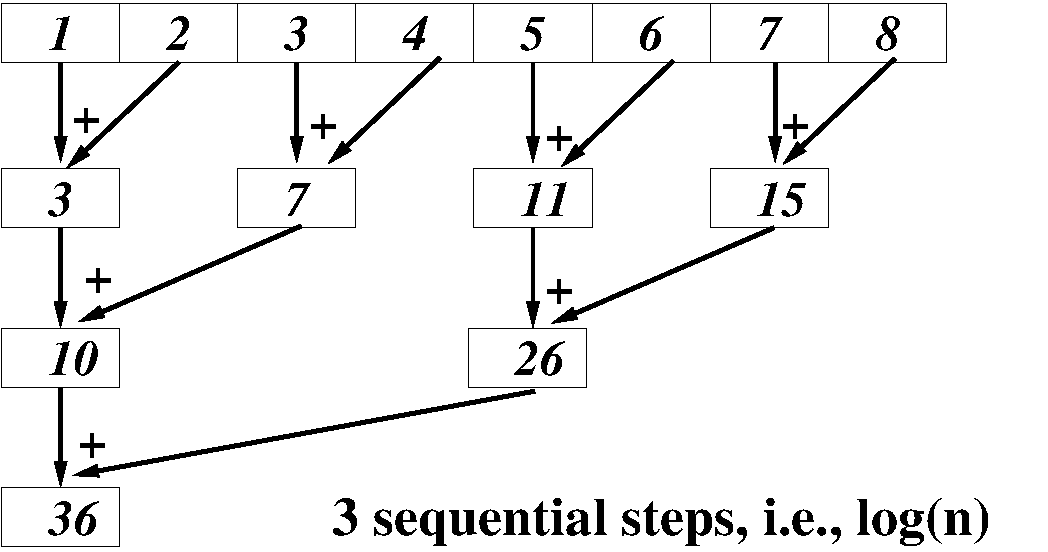
\includegraphics[height=25ex]{Figures/ReduceEg.pdf} 
\end{center} 

Build programs by combining \emp{map}, \emp{reduce} and other such operators. %Example: \smallskip

\end{frame}


\begin{frame}[fragile,t]
  \frametitle{1st List-Homomorphism Theorem [Meertens]}

\begin{columns}
\column{0.45\textwidth}
\begin{colorcode}[fontsize=\small]
h( [ ] )   = e
h( [x] )   = f(x)
h( x ++ y) = h(x) \mymath{\odot} h(y)
\end{colorcode}
\column{0.52\textwidth}
\begin{colorcode}[fontsize=\small]
h    \mymath{\equiv}    reduce(\mymath{\odot}, e) \mymath{\circ} 
           map(f)
\end{colorcode}
\end{columns}
\medskip

\emp{\bf Important Note: $\odot$ needs to be associative and $e$ needs to be the neutral element of $\odot$!}
\bigskip
\pause

\begin{columns}
\column{0.45\textwidth}
\begin{colorcode}[fontsize=\small]
-- one :: Int -> Int,one(x)=1
len :: [T] -> Int
len([ ])    = \emp{0}
len([x])    = \emp{one}(x) \blue{-- \mymath{\equiv} 1}
len(x ++ y) = len(x) \emp{+} len(y)
\end{colorcode}
\column{0.52\textwidth}
\begin{colorcode}[fontsize=\small]
len \mymath{\equiv}\pause    reduce(+, 0) \mymath{\circ} 
          map(one)
\end{colorcode}
\end{columns}


\bigskip
\begin{columns}
\column{0.45\textwidth}
\begin{colorcode}[fontsize=\small]
all\mymath{\myindx{p}}([ ])  = True
all\mymath{\myindx{p}}([x])  = p(x) 
all\mymath{\myindx{p}}(x++y) = all\mymath{\myindx{p}}(x) && all\mymath{\myindx{p}}(y)
\end{colorcode}
\column{0.52\textwidth}
\begin{colorcode}[fontsize=\small]
all\mymath{\myindx{p}} \mymath{\equiv}\pause    reduce(&&, True) \mymath{\circ} 
           map(p)
\end{colorcode}
\end{columns}


\end{frame}


\begin{frame}[fragile,t]
  \frametitle{Conclusion}

What have we talked about today?\bigskip
\begin{itemize}
    \item Hardware Parallelism:\pause\\ the only way of scalably increasing the compute power.\bigskip
    \item Big Challenge:\pause having parallel commodity software.\bigskip
    \item List-Homomorphism:\\ a way of reasoning about parallelism and\\ of building inherently parallel programs.  
\end{itemize}
\end{frame}


\end{document}
